\chapter{Introduction}
In this chapter the targeted problem, along with the proposed solution will be introduced. To better understand the explored problem, 
key relevant background concepts will be introduced.

    \section{RoboCup}
    RoboCup is an attempt to advance the field of robotics by providing a common problem and an environment for sharing knowledge and collaborate.
    The Objective of RoboCup is to achieve fully autonomous soccer playing robots that are able to defeat the FIFA World Cup champions by 2050. 

    RoboCup has since evolved from just soccer and now includes multiple fields, Rescue, Soccer, @Home, Industrial and Junior.
    \cite{RoboCup}

    \section{Soccer League}
    RoboCup Soccer is split into multiple leagues, each with different challenges and focuses. The Small Size league uses small wheeled robots, 
    each team is composed of six robots and play using a orange golf ball while tracked by a top-view camera;
    This enables the robots to abstract from challenges such as complex vision detection, 
    walking and others, enabling the teams to focus on strategy and multi-robot/agent cooperation and 
    control in a highly dynamic environment with a hybrid centralized/distributed system. 

    Middle size League assimilates to small size league, but in this case, the robots are of a larger size and must have all sensors on board; 
    The main focus of the league is on mechatronics design, control and multi-agent cooperation at plan and perception levels.

    RoboCup also has simulation for most of its leagues, allowing the teams to focus on software and avoid the difficulties originated by using real robots hardware.

    The Standard Platform is a step-up from the simulation league as while it uses real robots, NAOs, it allows the teams to focus mainly on software while using real robots and the challenges of using real robots without having to develop custom hardware. Each robot is fully autonomous and takes its one decisions.

    The Humanoid league, assimilates the most to humans, using robots assimilating its shape and unlike robots outside the Humanoid League, the task of perception and world modeling is not simplified by using non-human like range sensors, making this, the most transversal league, requiring hardware and software development. 
    In addition to soccer competitions technical challenges take place. 
    Dynamic walking, running, and kicking the ball while maintaining balance, visual perception of the ball, other players, and the field, self-localization, and team play are among the many research issues investigated in the Humanoid League.
    % TODO: add links to pages and explain difference between humanoid sizes 

    \section{Bold Hearts}
    The Bold Hearts are the RoboCup team from the University of Hertfordshire. The team researches and develops software and hardware in the Humanoid league, specifically in the teen size league.
    The robots used by the team are based on the Darwin-OP but incrementally developed using custom 3D printed parts and a new computing unit, Odroid-XU4 and camera, the Logitech C920 Pro. 
    The Robots use ROS2 as an operating system.
    \cite{boldhearts}
    \begin{figure}[H]
        \centering
        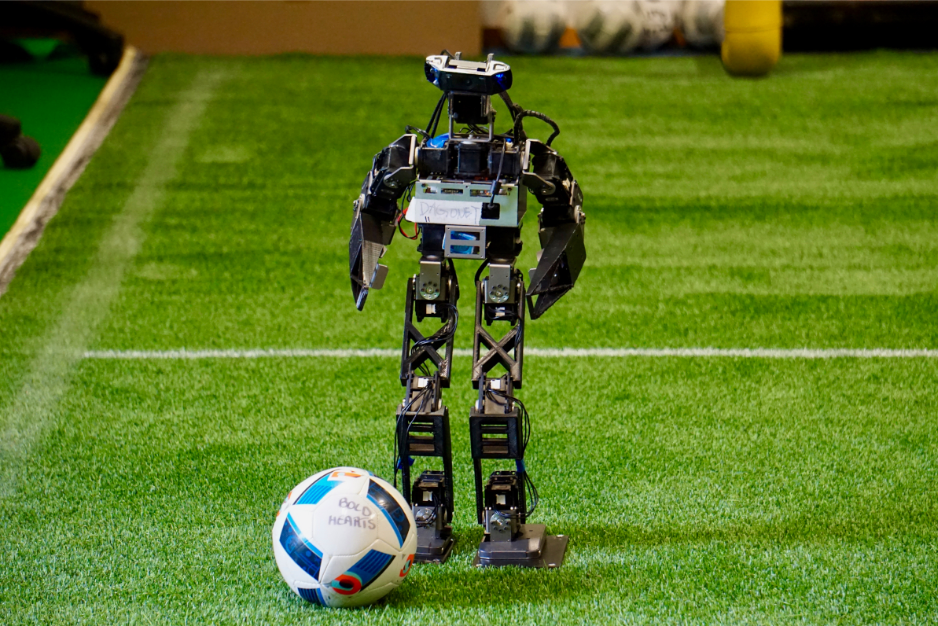
\includegraphics[scale=0.26]{figures/boldbot_2.png}
        \caption{Boldbot}
    \end{figure}

    \section{Introduction to the Project}

        \subsection{Problem}
        Robotic locomotion has, until a few years ago, been focused on wheel-based movement. Although it is very stable and easy to implement, it lacks flexibility, the ability to move on uneven, unpredictable terrain and overcome obstacles such as stairs.

        As a member of the Bold Hearts team our robots must be able to walk and, in addition to the high complexity of this challenges, 
        RoboCup rules periodically change, these changes are put in place as the RoboCup objective is to achieve the most realistic environment. 
        Rule changes affect both robots, changing the required height, sensors and others, as well as affecting the environment such as moving from flat ground to synthetic grass.

        One of the main challenges faced by the team is walking, which is one of the most complex movements performed by humans, requiring simultaneous control of multiple joints to move while maintaining balance. 
        This is one of the most energy and time-consuming problems faced by the team agravated by the rules changes and continuous improvements this requires updates to the robot's structural architecture, leading to new updates to the walking algorithm.

        \subsection{Proposed Solution}

        Walking algorithms can be developed using various techniques, 
        including explicit programming, supervised learning and unsupervised learning. 
        Walking is very complex as there are a lot of variables involved in it, such as the ground contact, 
        maintaining balance and the complex gait movement. The two main aspects important to highlight are that the walking algorithm requires changes when both the robot or external factors change and that it requires manual work from the team to achieve this. %TODO:probably double check how this are adapted

        The best way to solve the first mentioned problem requires having a robot and environment agnostic approach, this is possible by using Reinforcement Learning as the principles of the movement maintains therefore it should be possible to develop an agnostic reward function.
        From the moment a reinforcement learning solution is successfully implemented, the team should be able to use the same implementation to retrain the policy using the updated robot/environment that has been modeled in the simulator.
        This also allows to reduce the complexity of the problem as the input into the system is sensory data and the output is a set of actions to execute on the joints.

        \subsection{Aims and Objectives}
        This project proposes to develop a reinforcement learning implementation for walking, 
        to achieve the objectives of the project, three main topics will be covered, 
        robotics biped locomotion, reinforcement learning algorithms and the training framework.

        While achieving a working walking pattern would be desireable, the project aims to develop an implementation of reinforcement learning to achieve walking, 
        along with it aims to develop resourcefull documentation on the process and its results, allowing for reproducibility and further development and 
        adaptations of the current implementation to learn not only walking but any suitable problem.